% -*- mode: Latex; fill-column: 120; -*-
\documentclass{article}\usepackage[]{graphicx}\usepackage[]{color}
%% maxwidth is the original width if it is less than linewidth
%% otherwise use linewidth (to make sure the graphics do not exceed the margin)
\makeatletter
\def\maxwidth{ %
  \ifdim\Gin@nat@width>\linewidth
    \linewidth
  \else
    \Gin@nat@width
  \fi
}
\makeatother

\definecolor{fgcolor}{rgb}{0.345, 0.345, 0.345}
\newcommand{\hlnum}[1]{\textcolor[rgb]{0.686,0.059,0.569}{#1}}%
\newcommand{\hlstr}[1]{\textcolor[rgb]{0.192,0.494,0.8}{#1}}%
\newcommand{\hlcom}[1]{\textcolor[rgb]{0.678,0.584,0.686}{\textit{#1}}}%
\newcommand{\hlopt}[1]{\textcolor[rgb]{0,0,0}{#1}}%
\newcommand{\hlstd}[1]{\textcolor[rgb]{0.345,0.345,0.345}{#1}}%
\newcommand{\hlkwa}[1]{\textcolor[rgb]{0.161,0.373,0.58}{\textbf{#1}}}%
\newcommand{\hlkwb}[1]{\textcolor[rgb]{0.69,0.353,0.396}{#1}}%
\newcommand{\hlkwc}[1]{\textcolor[rgb]{0.333,0.667,0.333}{#1}}%
\newcommand{\hlkwd}[1]{\textcolor[rgb]{0.737,0.353,0.396}{\textbf{#1}}}%
\let\hlipl\hlkwb

\usepackage{framed}
\makeatletter
\newenvironment{kframe}{%
 \def\at@end@of@kframe{}%
 \ifinner\ifhmode%
  \def\at@end@of@kframe{\end{minipage}}%
  \begin{minipage}{\columnwidth}%
 \fi\fi%
 \def\FrameCommand##1{\hskip\@totalleftmargin \hskip-\fboxsep
 \colorbox{shadecolor}{##1}\hskip-\fboxsep
     % There is no \\@totalrightmargin, so:
     \hskip-\linewidth \hskip-\@totalleftmargin \hskip\columnwidth}%
 \MakeFramed {\advance\hsize-\width
   \@totalleftmargin\z@ \linewidth\hsize
   \@setminipage}}%
 {\par\unskip\endMakeFramed%
 \at@end@of@kframe}
\makeatother

\definecolor{shadecolor}{rgb}{.97, .97, .97}
\definecolor{messagecolor}{rgb}{0, 0, 0}
\definecolor{warningcolor}{rgb}{1, 0, 1}
\definecolor{errorcolor}{rgb}{1, 0, 0}
\newenvironment{knitrout}{}{} % an empty environment to be redefined in TeX

\usepackage{alltt}

\usepackage[letterpaper,margin=1in]{geometry}
\usepackage[breaklinks=true,colorlinks=true,urlcolor=blue]{hyperref}
\usepackage{bookmark}
\usepackage{times}
\usepackage{amsmath}
%\usepackage{graphicx}\usepackage[]{color}  knitr adds these
\IfFileExists{upquote.sty}{\usepackage{upquote}}{}
\begin{document}
\title{Fig 2 for Paper: Build 2A and 2B Glued Together}
\maketitle

\tableofcontents

\section{Intro}
2017-07-18: 
Initially we built Fig2A and Fig2B in different scripts (Fig2A-desert-distribution.rnw and nc-snps.rnw, resp.).  To streamline paper production and figure-tweaking, I've changed those two scripts to save the figure-relevant data they calculate into two .rda files that are loaded here, so that I can generate both figs together.  Most of the documentation about the figures remains in those scripts, but visual parameters (sizes, colors, ...) can all be set here.

\section{Preliminaries}
Load utility R code; do setup:

% setup.my.knitr includes opts_chunk$set(size='footnotesize'), but needed 1st time.
\begin{knitrout}\footnotesize
\definecolor{shadecolor}{rgb}{0.969, 0.969, 0.969}\color{fgcolor}\begin{kframe}
\begin{alltt}
\hlkwd{source}\hlstd{(}\hlstr{'../../../R/wlr.R'}\hlstd{)} \hlcom{# load util code; path relative this folder or sibling in scripts/larrys }
\end{alltt}
\begin{verbatim}
## Running as: ruzzo @ recycle.cs.washington.edu; SVN Id, I miss you.  $Id: wlr.R  2017-07-21 or later $
\end{verbatim}
\begin{alltt}
\hlkwd{setup.my.wd}\hlstd{(}\hlstr{'paperfigs'}\hlstd{)} \hlcom{# set working dir; UPDATE if this file moves, or if COPY/PASTE to new file}
\hlkwd{setup.my.knitr}\hlstd{(}\hlstr{'Fig2-glue-figs-knitr/'}\hlstd{)} \hlcom{# knitr's "unnamed-chunk-nnn" figures}
\hlstd{my.figs.dir} \hlkwb{<-} \hlstr{'Fig2-glue-figs-mine/'}   \hlcom{# my named figures}
\hlkwd{generic.setup}\hlstd{(my.figs.dir)}
\end{alltt}
\end{kframe}
\end{knitrout}
\begin{knitrout}\footnotesize
\definecolor{shadecolor}{rgb}{0.969, 0.969, 0.969}\color{fgcolor}\begin{kframe}
\begin{alltt}
\hlcom{# frequently need to add figpath to file name}
\hlstd{fpath} \hlkwb{<-} \hlkwa{function}\hlstd{(}\hlkwc{base}\hlstd{,} \hlkwc{suffix}\hlstd{=}\hlstr{'.pdf'}\hlstd{,} \hlkwc{dir}\hlstd{=my.figs.dir)\{}
  \hlkwd{return}\hlstd{(}\hlkwd{paste}\hlstd{(dir, base, suffix,} \hlkwc{sep}\hlstd{=}\hlstr{''}\hlstd{))}
\hlstd{\}}
\end{alltt}
\end{kframe}
\end{knitrout}

\section{Setup for Fig 2A}

\begin{knitrout}\footnotesize
\definecolor{shadecolor}{rgb}{0.969, 0.969, 0.969}\color{fgcolor}\begin{kframe}
\begin{alltt}
\hlstd{chr1.len} \hlkwb{<-} \hlkwd{genome.length.constants}\hlstd{()}\hlopt{$}\hlstd{chr1.length}  \hlcom{## 3042585}
\hlkwd{load}\hlstd{(}\hlstr{'Fig2A-data.rda'}\hlstd{)}           \hlcom{# contains the "gap table" all.n.na}
\hlkwd{load}\hlstd{(}\hlstr{'../../../data/des.rda'}\hlstd{)}    \hlcom{# desert tables from svn+ssh://ceg1.ocean.washington.edu/var/svn/7_strains/trunk/code/snpNB/data}
\hlkwd{names}\hlstd{(des)[[}\hlnum{6}\hlstd{]]} \hlkwb{<-} \hlstr{'tp3367'}      \hlcom{# override oldschool name}
\hlstd{strain.order} \hlkwb{<-} \hlkwd{c}\hlstd{(}\hlnum{7}\hlstd{,}\hlnum{1}\hlstd{,}\hlnum{2}\hlstd{,}\hlnum{5}\hlstd{,}\hlnum{4}\hlstd{,}\hlnum{3}\hlstd{,}\hlnum{6}\hlstd{)} \hlcom{# Order of isolates, top-to-bottom in fig 2A}
\end{alltt}
\end{kframe}
\end{knitrout}

\section{Setup for Fig 2B}

\begin{knitrout}\footnotesize
\definecolor{shadecolor}{rgb}{0.969, 0.969, 0.969}\color{fgcolor}\begin{kframe}
\begin{alltt}
\hlkwd{load}\hlstd{(}\hlstr{'../nc-snps/Fig2B-data.rda'}\hlstd{)} \hlcom{# provides snp.rates.blob, needed by snp.rates.plot}
\end{alltt}
\end{kframe}
\end{knitrout}

\section{Create Plot}

\begin{knitrout}\footnotesize
\definecolor{shadecolor}{rgb}{0.969, 0.969, 0.969}\color{fgcolor}\begin{kframe}
\begin{alltt}
\hlstd{heights.a.b} \hlkwb{<-} \hlkwd{c}\hlstd{(}\hlnum{2.7}\hlstd{,} \hlnum{1.8}\hlstd{)} \hlcom{# panel heights (inches)}
\hlkwd{pdf}\hlstd{(}\hlkwd{fpath}\hlstd{(}\hlstr{'Fig2'}\hlstd{),}\hlkwc{width}\hlstd{=}\hlnum{6.5}\hlstd{,} \hlkwc{height}\hlstd{=}\hlkwd{sum}\hlstd{(heights.a.b))}
\hlstd{opar} \hlkwb{<-} \hlkwd{par}\hlstd{(}\hlkwc{no.readonly}\hlstd{=}\hlnum{TRUE}\hlstd{,} \hlkwc{oma}\hlstd{=}\hlkwd{c}\hlstd{(}\hlnum{0}\hlstd{,}\hlnum{0}\hlstd{,}\hlnum{0}\hlstd{,}\hlnum{0}\hlstd{),} \hlkwc{mar}\hlstd{=}\hlkwd{c}\hlstd{(}\hlnum{3}\hlstd{,}\hlnum{3}\hlstd{,}\hlnum{0.4}\hlstd{,}\hlnum{0.4}\hlstd{),} \hlkwc{tcl}\hlstd{=}\hlopt{-}\hlnum{0.2}\hlstd{)}
\hlkwd{layout}\hlstd{(}\hlkwd{matrix}\hlstd{(}\hlnum{1}\hlopt{:}\hlnum{2}\hlstd{,}\hlkwc{nrow}\hlstd{=}\hlnum{2}\hlstd{),} \hlkwc{heights}\hlstd{=heights.a.b)}

\hlcom{# Fig 2A:}
\hlkwd{draw.des.fig}\hlstd{(des, all.n.na,} \hlkwc{width}\hlstd{=chr1.len,} \hlkwc{row.order}\hlstd{=strain.order,} \hlkwc{panel.label}\hlstd{=}\hlstr{'A'}\hlstd{,} \hlkwc{chr}\hlstd{=}\hlstr{'Chr1'}\hlstd{,}
             \hlkwc{xlab}\hlstd{=}\hlstr{'Chromosome 1 Position (Mb)'}\hlstd{,} \hlkwc{gap.col} \hlstd{=} \hlstr{'gold'}\hlstd{,} \hlkwc{d.col}\hlstd{=}\hlstr{'dodgerblue2'}\hlstd{,}
             \hlkwc{min.des}\hlstd{=}\hlnum{10000}\hlstd{,} \hlkwc{twotone}\hlstd{=}\hlstr{'lightblue'}\hlstd{,} \hlkwc{do.par}\hlstd{=}\hlnum{FALSE}\hlstd{)}

\hlcom{# Fig 2B:}
\hlstd{xx} \hlkwb{<-} \hlkwd{snp.rates.plot}\hlstd{(snp.rates.blob,} \hlkwc{des.col}\hlstd{=}\hlstr{'blue3'}\hlstd{,} \hlkwc{undes.col}\hlstd{=}\hlstr{'black'}\hlstd{,} \hlkwc{yclip}\hlstd{=}\hlnum{0.01}\hlstd{,} \hlkwc{legend}\hlstd{=}\hlstr{''}\hlstd{,}
                     \hlkwc{xlab}\hlstd{=}\hlstr{'Desert Index'}\hlstd{,} \hlkwc{ylab}\hlstd{=}\hlstr{'SNP Density'}\hlstd{,} \hlkwc{main}\hlstd{=}\hlstr{''}\hlstd{,}
                     \hlkwc{ylab.sub}\hlstd{=}\hlkwd{list}\hlstd{(}\hlkwc{text}\hlstd{=}\hlstr{'(SNPS / bp)'}\hlstd{,} \hlkwc{line}\hlstd{=}\hlnum{1.1}\hlstd{,} \hlkwc{cex}\hlstd{=}\hlnum{.75}\hlstd{),}
                     \hlkwc{yticks}\hlstd{=}\hlkwd{list}\hlstd{(}\hlkwc{padj}\hlstd{=}\hlnum{1.6}\hlstd{,} \hlkwc{at}\hlstd{=}\hlkwd{seq}\hlstd{(}\hlnum{0}\hlstd{,}\hlnum{0.01}\hlstd{,}\hlnum{0.0025}\hlstd{),}
                                 \hlkwc{labels}\hlstd{=}\hlkwd{c}\hlstd{(}\hlstr{'0.000'}\hlstd{,}\hlstr{''}\hlstd{,}\hlstr{'0.005'}\hlstd{,}\hlstr{''}\hlstd{,}\hlstr{'0.010'}\hlstd{),} \hlkwc{cex}\hlstd{=}\hlnum{.9}\hlstd{))}
\hlcom{# panel='B':}
\hlkwd{text}\hlstd{(}\hlnum{0.62}\hlstd{,}\hlnum{0.0092}\hlstd{,}\hlstr{'B'}\hlstd{,}\hlkwc{cex}\hlstd{=}\hlnum{1.1}\hlstd{)} \hlcom{# for 2B, coords empirically set to roughly match rel pos in panel 2A}

\hlkwd{dev.off}\hlstd{()}
\end{alltt}
\begin{verbatim}
# pdf 
#   2
\end{verbatim}
\begin{alltt}
\hlkwd{par}\hlstd{(opar)}
\end{alltt}
\end{kframe}
\end{knitrout}

Fig~\ref{fig:2a2b} shows it.  (Surrounding boxes just to make marginal space obvious; change fbox to mbox to remove.)
\begin{figure}
  \begin{center}
    %\fbox{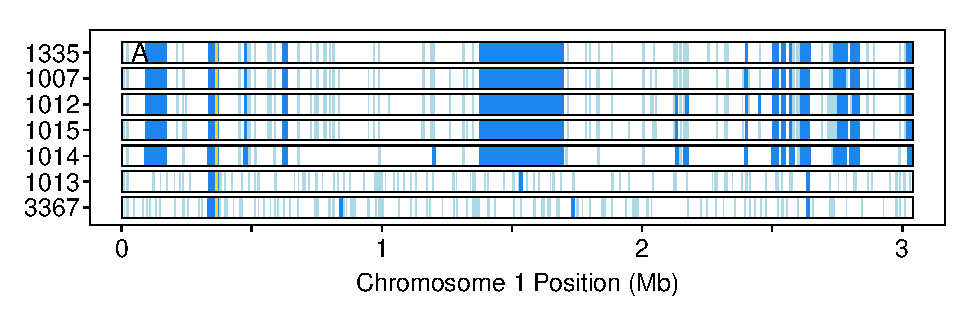
\includegraphics{Fig2A-desert-distribution-figs-mine/Fig2A-desert-distribution-figq.pdf}}\\
    %\fbox{\includegraphics{../../../inst/doc/figures4paper/Fig2B-bigdes-snpdens-ny.pdf}}
    \fbox{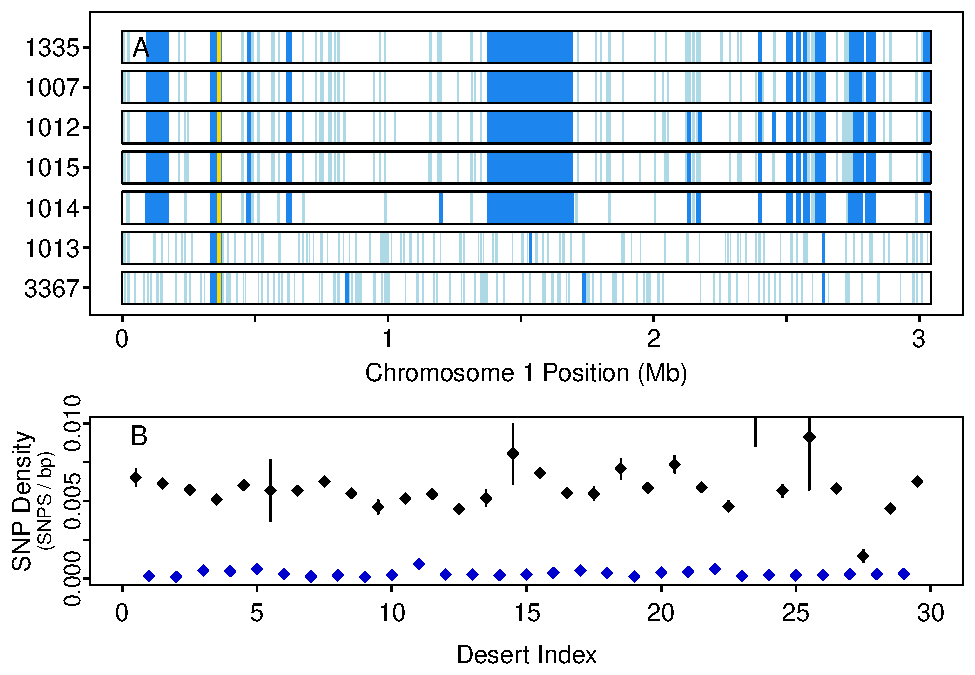
\includegraphics{Fig2-glue-figs-mine/Fig2.pdf}}
  \end{center}
  \caption{Proposed caption: Attributes of SNP deserts for {\it T. pseudonana\/} isolates. A) SNP distributions across the 3 Mb of Chromosome 1 for the seven {\it T. pseudonana\/} isolates. Regions in blue have significantly low SNP density (``SNP deserts'') based on a negative binomial model (Methods). Pink(???) region is a gap of known size in the reference sequence. The large region centered near 1.5Mb is a 320Kb SNP desert present in all L-isolates but neither H-isolate. B) SNP densities (SNP per base-pair---$\mu\pm2\sigma$) in the 29 deserts that span at least 50Kb of the CCMP 1335 genome (blue) and the thirty regions surrounding these deserts (including deserts smaller than 50Kb; black).  }
  \label{fig:2a2b}
\end{figure}

\vfill\footnotesize\flushright SVN ID I miss you $ $Id: Fig2.rnw 2017-07-20 or later ruzzo $ $
\end{document}
